%!Mode:: "TeX:UTF-8"
\documentclass[a4paper,11pt,UTF8]{ctexart}

\usepackage{indentfirst} %缩进
\usepackage{xeCJK}    %使用系统字体
\usepackage{fancyhdr} %自定义页眉页脚
\pagestyle{empty}                   %不设置页眉页脚
\usepackage{amsmath, amsthm, amssymb, amsfonts} %数学公式
\usepackage[a4paper,left=3cm,right=3cm,top=3cm,bottom=3cm]{geometry}
%\usepackage[tmargin=1in,bmargin=1in,lmargin=1.25in,rmargin=1.25in]{geometry}.
\usepackage{booktabs} %插入表格
\usepackage[section]{placeins} %避免浮动
\usepackage{listings} %插入代码
\usepackage{ctex}     %中文宏包
\usepackage[svgnames, table]{xcolor} %彩色表格
\usepackage{algorithm}          %伪代码
\usepackage{algorithmicx}
\usepackage{algpseudocode}
\usepackage{algorithm,algpseudocode,float}
\usepackage{lipsum}
\usepackage{enumitem}           %调整列举环境
\usepackage{url}
\usepackage{fontspec,xunicode}
\defaultfontfeatures{Mapping=tex-text} %如果没有它,会有一些 tex 特殊字符无法正常使用,比如连字符。

\usepackage{graphicx}
\graphicspath{{imgs/}}

%%%%%%%%%%%%%%%%%%%%%%%%%%%%%%%%%%%%%%%%%%%%%%%%%%%%%%%%%%%%%%%%
% 缩进及行间距
%%%%%%%%%%%%%%%%%%%%%%%%%%%%%%%%%%%%%%%%%%%%%%%%%%%%%%%%%%%%%%%%
\setlength{\parindent}{22pt} %重新定义缩进长度
\setlength{\baselineskip}{20pt}  %定义行间距
%\renewcommand{\baselinestretch}{1.1} %定义行间距

%%%%%%%%%%%%%%%%%%%%%%%%%%%%%%%%%%%%%%%%%%%%%%%%%%%%%%%%%%%%%%%%
% 列表设置
%%%%%%%%%%%%%%%%%%%%%%%%%%%%%%%%%%%%%%%%%%%%%%%%%%%%%%%%%%%%%%%%
\setenumerate{fullwidth,itemindent=\parindent,listparindent=\parindent,itemsep=0ex,partopsep=0pt,parsep=0ex}
\setenumerate[2]{label=\alph*),leftmargin=1.5em}  %二级item设置
\setitemize{itemindent=38pt,leftmargin=0pt,itemsep=-0.4ex,listparindent=26pt,partopsep=0pt,parsep=0.5ex,topsep=-0.25ex}
\setdescription{itemindent=38pt,leftmargin=0pt,itemsep=-0.4ex,listparindent=26pt,partopsep=0pt,parsep=0.5ex,topsep=-0.25ex}

%%%%%%%%%%%%%%%%%%%%%%%%%%%%%%%%%%%%%%%%%%%%%%%%%%%%%%%%%%%%%%%%
% 图的标题行间距设置
%%%%%%%%%%%%%%%%%%%%%%%%%%%%%%%%%%%%%%%%%%%%%%%%%%%%%%%%%%%%%%%%
\newcommand{\bottomcaption}{%
\setlength{\abovecaptionskip}{6pt}%
\setlength{\belowcaptionskip}{6pt}%
\caption}


%%%%%%%%%%%%%%%%%%%%%%%%%%%%%%%%%%%%%%%%%%%%%%%%%%%%%%%%%%%%%%%%
% 字体定义
%%%%%%%%%%%%%%%%%%%%%%%%%%%%%%%%%%%%%%%%%%%%%%%%%%%%%%%%%%%%%%%%
\setmainfont{Times New Roman}  %默认英文字体.serif是有衬线字体sans serif无衬线字体
\setmonofont{Consolas}
\setCJKmainfont[ItalicFont={楷体}, BoldFont={黑体}]{宋体}%衬线字体 缺省中文字体为
\setCJKsansfont{黑体}
\punctstyle{hangmobanjiao}
%-----------------------xeCJK下设置中文字体------------------------------%
\setCJKfamilyfont{song}{SimSun}                             %宋体 song
\newcommand{\song}{\CJKfamily{song}}
\setCJKfamilyfont{fs}{FangSong}                      %仿宋  fs
\newcommand{\fs}{\CJKfamily{fs}}
\setCJKfamilyfont{ktgb}{KaiTi}                      %楷体2312 ktgb
\newcommand{\ktgb}{\CJKfamily{ktgb}}
\setCJKfamilyfont{yh}{Microsoft YaHei}                    %微软雅黑 yh
\newcommand{\yh}{\CJKfamily{yh}}
\setCJKfamilyfont{hei}{SimHei}                              %黑体  hei
\newcommand{\hei}{\CJKfamily{hei}}
\setCJKfamilyfont{hwxk}{STXingkai}                                %华文行楷  hwxk
\newcommand{\hwxk}{\CJKfamily{hwxk}}
%------------------------------设置字体大小------------------------%
\newcommand{\shiyanbaogao}{\fontsize{36pt}{\baselineskip}\selectfont}
\newcommand{\chuhao}{\fontsize{42pt}{\baselineskip}\selectfont}     %初号
\newcommand{\xiaochuhao}{\fontsize{36pt}{\baselineskip}\selectfont} %小初号
\newcommand{\yihao}{\fontsize{28pt}{\baselineskip}\selectfont}      %一号
\newcommand{\erhao}{\fontsize{21pt}{\baselineskip}\selectfont}      %二号
\newcommand{\xiaoerhao}{\fontsize{18pt}{\baselineskip}\selectfont}  %小二号
\newcommand{\sanhao}{\fontsize{15.75pt}{\baselineskip}\selectfont}  %三号
\newcommand{\sihao}{\fontsize{14pt}{\baselineskip}\selectfont}       %四号
\newcommand{\xiaosihao}{\fontsize{12pt}{\baselineskip}\selectfont}  %小四号
\newcommand{\wuhao}{\fontsize{10.5pt}{\baselineskip}\selectfont}    %五号
\newcommand{\xiaowuhao}{\fontsize{9pt}{\baselineskip}\selectfont}   %小五号
\newcommand{\liuhao}{\fontsize{7.875pt}{\baselineskip}\selectfont}  %六号
\newcommand{\qihao}{\fontsize{5.25pt}{\baselineskip}\selectfont}    %七号

%%%%%%%%%%%%%%%%%%%%%%%%%%%%%%%%%%%%%%%%%%%%%%%%%%%%%%%%%%%%%%%%
% 图题字体大小相同
%%%%%%%%%%%%%%%%%%%%%%%%%%%%%%%%%%%%%%%%%%%%%%%%%%%%%%%%%%%%%%%%
\usepackage{caption}
\captionsetup{font={footnotesize}}   % footnotesize = 9pt
\captionsetup[lstlisting]{font={footnotesize}}

%%%%%%%%%%%%%%%%%%%%%%%%%%%%%%%%%%%%%%%%%%%%%%%%%%%%%%%%%%%%%%%%
% 重定义枚举编号为 1),2)...
%%%%%%%%%%%%%%%%%%%%%%%%%%%%%%%%%%%%%%%%%%%%%%%%%%%%%%%%%%%%%%%%
\renewcommand{\labelenumi}{\theenumi)}

%%%%%%%%%%%%%%%%%%%%%%%%%%%%%%%%%%%%%%%%%%%%%%%%%%%%%%%%%%%%%%%%
% 标题名称中文化
%%%%%%%%%%%%%%%%%%%%%%%%%%%%%%%%%%%%%%%%%%%%%%%%%%%%%%%%%%%%%%%%
\renewcommand\figurename{\hei 图}
\renewcommand\tablename{\hei 表}
\renewcommand\lstlistingname{\hei 代码}
\renewcommand{\algorithmicrequire}{\textbf{输入:}}
\renewcommand{\algorithmicensure}{\textbf{输出:}}
\newtheorem{define}{定义}

%%%%%%%%%%%%%%%%%%%%%%%%%%%%%%%%%%%%%%%%%%%%%%%%%%%%%%%%%%%%%%%%
% 代码设置
%%%%%%%%%%%%%%%%%%%%%%%%%%%%%%%%%%%%%%%%%%%%%%%%%%%%%%%%%%%%%%%%
\lstset{
 columns=fixed,
 numbers=left,                                        % 在左侧显示行号
 numberstyle=\tiny\color{gray},                       % 设定行号格式
 frame=single,                                        % 单线背景边框
 breaklines=true,                                     % 设定LaTeX对过长的代码行进行自动换行
 keywordstyle=\color[RGB]{40,40,255},                 % 设定关键字颜色
 numberstyle=\footnotesize\color{darkgray},
 commentstyle=\it\color[RGB]{0,96,96},                % 设置代码注释的格式
 stringstyle=\rmfamily\slshape\color[RGB]{128,0,0},   % 设置字符串格式
 showstringspaces=false,                              % 不显示字符串中的空格
 language=java,                                        % 设置语言
 basicstyle=\linespread{1.0}\xiaowuhao\ttfamily,                      % 字体字号
 %lineskip=10pt,
 %baselinestretch=1,
}

%%%%%%%%%%%%%%%%%%%%%%%%%%%%%%%%%%%%%%%%%%%%%%%%%%%%%%%%%%%%%%%%
% 伪代码分页
%%%%%%%%%%%%%%%%%%%%%%%%%%%%%%%%%%%%%%%%%%%%%%%%%%%%%%%%%%%%%%%%
\makeatletter
\renewcommand{\ALG@name}{算法}
\newenvironment{breakablealgorithm}
  {% \begin{breakablealgorithm}
   \begin{center}
     \refstepcounter{algorithm}% New algorithm
     \hrule height.8pt depth0pt \kern2pt% \@fs@pre for \@fs@ruled
     \renewcommand{\caption}[2][\relax]{% Make a new \caption
       {\raggedright\textbf{\ALG@name~\thealgorithm} ##2\par}%
       \ifx\relax##1\relax % #1 is \relax
         \addcontentsline{loa}{algorithm}{\protect\numberline{\thealgorithm}##2}%
       \else % #1 is not \relax
         \addcontentsline{loa}{algorithm}{\protect\numberline{\thealgorithm}##1}%
       \fi
       \kern2pt\hrule\kern2pt
     }
  }{% \end{breakablealgorithm}
     \kern2pt\hrule\relax% \@fs@post for \@fs@ruled
   \end{center}
  }
\makeatother

% =============================================
% Part 1 Edit the info
% =============================================

\newcommand{\major}{物理学院}
\newcommand{\name}{黄阅迅,李秋阳}
\newcommand{\stuid}{PB18020631,PB18020567}
\newcommand{\group}{20}
\newcommand{\newdate}{\today}


\newcommand{\course}{电子线路实验(1)}
\newcommand{\newtitle}{负反馈放大器的研究}

% =============================================
% Part 1 Main document
% =============================================
\begin{document}
\thispagestyle{empty}
\begin{figure}[h]
  \begin{minipage}{0.6\linewidth}
    \centerline{
\includegraphics[width=\linewidth]{logo.png}}
  \end{minipage}
  \hfill
  \begin{minipage}{.4\linewidth}
    \raggedleft
    \begin{tabular*}{.8\linewidth}{ll}
      学院: & \underline\major   \\
      姓名: & \underline\name    \\
      学号: & \underline\stuid   \\
      组号:  & \underline\group   \\
      日期: & \underline\newdate \\
    \end{tabular*}
  \end{minipage}
\end{figure}

\begin{table}[!htbp]
  \centering
  \begin{tabular*}{\linewidth}{llllll}
    课程名称:  \underline\course   \qquad\qquad 实验题目:  \underline\newtitle  
  \end{tabular*}
\end{table}

% =============================================
% Part 2 Main document
% =============================================

\section{实验目的}

请参见预习报告。

\section{实验原理}

请参见预习报告。

\section{实验内容与步骤}
\subsection{实验内容1}
	测量基本放大器的静态工作点以及动态参数。
\subsection{实验步骤1}
	\begin{enumerate}
    \item 连接好基本放大器线路图如图 \ref{fig:basicCircuit}所示。注意需考虑负载效应。
    \item 输入断路,输出开路,调节$100k\Omega$电位器使得第二级的$I_{C2}=1.0mA$,用万用表测量两级放大电路的静态工作点。
    \item 输入接入$f=1kHz,U_i=20mVrms$的正弦交流电路,分别测量空载和$10k\Omega$负载下的输出,计算增益系数和输出电阻,并用示波器观察相位。
    \item 接入负载,固定输入电压为$20mVrms$,改变输入信号频率,测量出其上截止与下截止频率。
    \item 接入负载,输入中串入电阻$R=2k\Omega$,测量出$U_s,U_i$,计算输入电阻。
  \end{enumerate}
  \begin{figure}[htbp]
    \centering
    \fbox{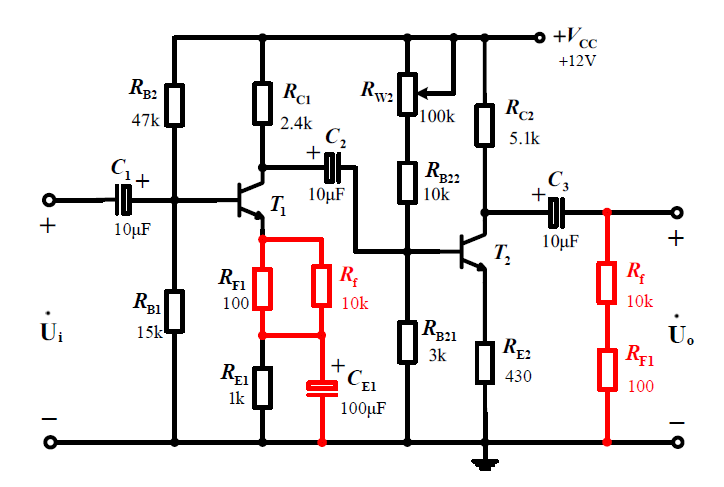
\includegraphics[width=0.5\linewidth]{basicCircuit.png}}
    \caption{考虑负载效应的基本放大器线路图}
    \label{fig:basicCircuit}
    \end{figure}

    \subsection{实验内容2}
    测量负基本放大器的静态工作点以及动态参数。
  \subsection{实验步骤2}
    \begin{enumerate}
      \item 连接好基本放大器线路图如图 \ref{fig:feedbackCircuit}所示。
      \item 输入接入$f=1kHz,U_i=20mVrms$的正弦交流电路,分别测量空载和$10k\Omega$负载下的输出,计算增益系数和输出电阻,并用示波器观察相位。
      \item 接入负载,固定输入电压为$20mVrms$,改变输入信号频率,测量出其上截止与下截止频率。
      \item 接入负载,输入中串入电阻$R=2k\Omega$,测量出$U_s,U_i$,计算输入电阻。
    \end{enumerate}
    \begin{figure}[htbp]
      \centering
      \fbox{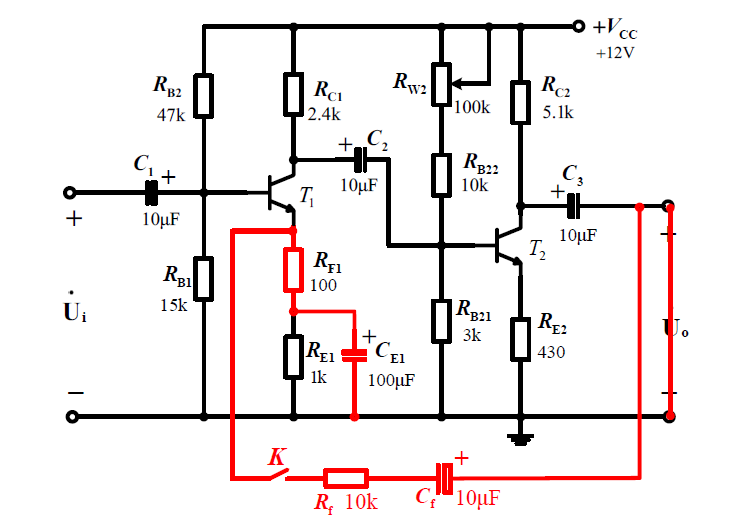
\includegraphics[width=0.5\linewidth]{feedbackCircuit.png}}
      \caption{负反馈放大器线路图}
      \label{fig:feedbackCircuit}
      \end{figure}

\section{实验数据处理与分析}
\subsection{实验内容1}
  \subsubsection{静态工作点}
  实验测量得到的静态工作点如表 \ref{tab:tab1}所示。可见测量得到的$I_{C2}$略有偏差。
  \begin{table}[!h!tbp]
    \caption{静态工作点数据}\label{tab:tab1}
      \centering
      \begin{tabular}{|l|c|c|c|c|c|}
      \hline
      级数        &$U_B(V)$   &$U_E(V)$ &$U_C(V)$ &$I_C(mA)$  &$R_{W2}$         \\ \hline
      一          &$2.64$     &$2.01$   &$7.46$   &$1.89$     &$20.50$\\ \hline
      二          &$1.04$     &$0.43$   &$6.65$   &$1.05$     &$20.50$\\ \hline
    \end{tabular}
    \end{table}
  \subsubsection{误差分析}
  下面理论计算静态工作点数据,以下计算取$r_{bb'}=300\Omega,\beta=150,U_{BE}=0.7V$。
  \begin{equation}
    \begin{aligned}
      U_{B1}&=V_{CC}\frac{R_{B1}}{R_{B2}+R_{B1}}=2.90V\\
      U_{E1}&=U_{B1}-U_{BE}=2.20V\\
      I_{C1}&\approx I_{E1}=\frac{U_{E1}}{R_{F1}\parallel R_{f}+R_{E1}}=2.00mA\\
      U_{C1}&=V_{CC}-I_C R_{C1}=7.20V\\
      &\,\\
      U_{B2}&=V_{CC}\frac{R_{B1}}{R_{W2}+R_{B22}+R_{B21}}=1.07V\\
      U_{E2}&=U_{B2}-U_{BE}=0.37V\\
      I_{C2}&\approx I_{E2}=\frac{U_{E2}}{R_{E2}}=0.86mA\\
      U_{C2}&=V_{CC}-I_C R_{C2}=7.61V\\
    \end{aligned}
  \end{equation}
  则对应的可以算出各个量的相对误差以及采用实验测得的数据计算的$r_{be}$如下:
  \begin{equation}
    \begin{aligned}
      \left |\frac{\Delta U_{B1}}{U_{B1}}\right |&=9.0\%,
      \left |\frac{\Delta U_{E1}}{U_{E1}}\right |&=8.6\%,
      \left |\frac{\Delta U_{C1}}{U_{C1}}\right |&=3.6\%,
      \left |\frac{\Delta I_{C1}}{I_{C1}}\right |&=5.5\%\\ 
      \left |\frac{\Delta U_{B2}}{U_{B2}}\right |&=2.8\%,
      \left |\frac{\Delta U_{E2}}{U_{E2}}\right |&=16\%,
      \left |\frac{\Delta U_{C2}}{U_{C2}}\right |&=13\%,
      \left |\frac{\Delta I_{C2}}{I_{C2}}\right |&=22\%\\
    \end{aligned}
  \end{equation}
  \begin{equation}
    \begin{aligned}
      r_{be1}&=r_{bb'}+(1+\beta)\frac{26mV}{I_E(mA)}=2.37k\Omega\\
      r_{be2}&=r_{bb'}+(1+\beta)\frac{26mV}{I_E(mA)}=4.04k\Omega\\
    \end{aligned}
  \end{equation}
  可见第一级的误差较低,而第二级的误差较大,这个误差从第一级的数据中可以看出,应该主要是元件的参数不准确造成的。但本身分压
  计算就是一种近似,因此也有这方面带来的误差。同时观察数据还可以得到,三极管的数据$U_{BE}=0.7V$这个值应该有所偏差,两个管的值可能是$0.6V$,但修正不大,因为$U_B$的计算本身就不准确。
  \subsubsection{增益以及输出输入电阻}
  实验测量得到的$1kHz$下两种负载条件下的输出增益以及电阻如表 \ref{tab:tab2}所示。输出电压经示波器观察均与输入同向。(输入电阻测量时的$U_S$与$U_i$已省略,请参见原始数据)
  \begin{table}[!h!tbp]
    \caption{动态参数数据}\label{tab:tab2}
      \centering
      \begin{tabular}{|l|c|c|c|c|c|}
      \hline
      $U_i(mVrms)$  &$R_L(k\Omega)$  &$U_O(V)$ &$A_u$   &$R_o(k\Omega)$  &$R_{i}(k\Omega)$         \\ \hline
      $19.7$        &$\infty$        &$1.53$   &$77.7$  &$3.42$          &$6.56$\\ \hline
      $19.7$        &$10$            &$1.14$   &$57.9$  &$3.42$          &$6.56$\\ \hline
    \end{tabular}
    \end{table}
    \subsubsection{误差分析}
    为了分析实验误差,需要先画出交流通路如图 \ref{fig:ACModel}所示。可见,级联的交流通路在分析时可以将后一级的输入电阻等效入前一级的负载。

    \begin{figure}[htbp]
      \centering
      \fbox{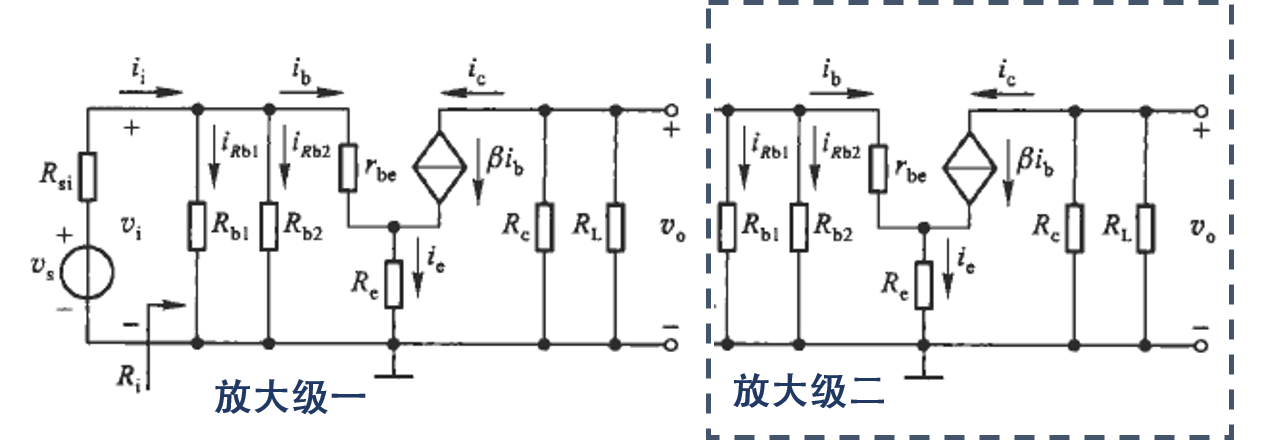
\includegraphics[width=0.8\linewidth]{ACModel.png}}
      \caption{交流通路图}
      \label{fig:ACModel}
      \end{figure}
    则理论分析如下:
    \begin{equation}
      \begin{aligned}
        R_{C2}'&=R_{C2}\parallel R_f=3.38k\Omega\\
        A_{v2}&=\frac{-\beta R_{C2'}\parallel R_L}{r_{be2}+(1+\beta)R_{E2}}\\
        A_{v2o}&=-7.35,A_{v2L}=-5.49\\
        R_o&=R_{o2}\approx R_{C2}'=3.38k\Omega\\
        R_{i2}&=(R_{B22}+R_{W2})\parallel R_{B21}\parallel [r_{be2}+(1+\beta)R_{C2}']= 2.63k\Omega\\
        &\,\\
        R_{C1}'&=R_{C1}\parallel R_{i2}=1.25k\Omega\\
        A_{v1}&=\frac{-\beta R_{C1'}}{r_{be1}+(1+\beta)(R_{F1}\parallel R_{f})}=-10.8\\
        A_{vo}&=79.6,A_{v2L}=56.4\\
        R_{i}&=R_{i1}=R_{B1}\parallel R_{B2}\parallel[r_{be1}+(1+\beta)(R_{F1}\parallel R_{f})]=6.86k\Omega
      \end{aligned}
    \end{equation}
    则可以计算出每个动态参数的相对误差为:
    \begin{equation}
      \begin{aligned}
        \left |\frac{\Delta A_{vo}}{A_{vo}}\right |=2.4\%,
        \left |\frac{\Delta A_{vL}}{A_{vL}}\right |=2.6\%,
        \left |\frac{\Delta R_{i}}{R_{i}}\right |=4.3\%,
        \left |\frac{\Delta R_{o}}{R_{o}}\right |=1.2\%
      \end{aligned}
    \end{equation}
    可见相对误差相当之小,比较理想,这是因为计算时采用的静态工作点的测量值来完成。而仍然由一定误差,这是因为交流通路本身就是一种
    近似模型,同时三极管的参数也有不准,实验采用的元件由于年久失修,其实真实值与标定值也有一定差异。
    \subsubsection{通频带}
    实验测量得到的通频带为$19.6Hz-320kHz$。带宽为$BW=320kHz$。下截值频率很小,而上截止频率相对不算特别大。
    \subsubsection{误差分析}
    通频带的测量误差主要有两个方面,第一个是读数误差,第二是调节函数发生器时实际上无法严格保证输入电压不变,因为调节的最小精度值不足以修正频率带来的误差。以上两者都带来了一定误差。本电路的带宽理论分析非常复杂而且
    缺少三极管参数,因此不作进一步分析。
  \subsection{实验内容2}
  \subsubsection{增益以及输出输入电阻}
  实验测量得到的$1kHz$下反馈电路两种负载条件下的输出增益以及电阻如表 \ref{tab:tab3}所示。输出电压经示波器观察均与输入同向。(输入电阻测量时的$U_S$与$U_i$已省略,请参见原始数据)
  \begin{table}[!h!tbp]
    \caption{反馈电路动态参数数据}\label{tab:tab3}
      \centering
      \begin{tabular}{|l|c|c|c|c|c|}
      \hline
      $U_i(mVrms)$  &$R_L(k\Omega)$  &$U_O(V)$  &$A_u$   &$R_o(k\Omega)$  &$R_{i}(k\Omega)$         \\ \hline
      $19.7$        &$\infty$        &$0.865$   &$43.9$  &$1.90$          &$9.67$\\ \hline
      $19.7$        &$10$            &$0.727$   &$36.9$  &$1.90$          &$9.67$\\ \hline
    \end{tabular}
    \end{table}
  可见增益变小,输出电阻减小,而输入电阻增大,基本符合理论预测。
  \subsubsection{误差分析}
  下面的计算均采用实验内容1中测量得到的普通放大电路的测量值进行计算。
  首先可以得到反馈系数:$F=\frac{R_{F1}}{R_{F1}+R_f}=9.9\times10^{-3}$
  则根据测量值可以计算出对应的动态参数:
  \begin{equation}
  \begin{aligned}
    R_{of}&=\frac{R_o}{1+A_{vo}F}=1.93k\Omega\\
    R_{if}&=R_i(1+A_{vL}F)=10.3k\Omega\\
    A_{vf}&=\frac{A_v}{1+FA_v}\\
    A_{vof}&=44.5,A_{vLf}=36.2
  \end{aligned}
  \end{equation}
  则可以计算出相对误差为:
  \begin{equation}
    \begin{aligned}
      \left |\frac{\Delta A_{vof}}{A_{vof}}\right |=1.3\%,
      \left |\frac{\Delta A_{vLf}}{A_{vLf}}\right |=1.9\%,
      \left |\frac{\Delta R_{if}}{R_{if}}\right |=6.1\%,
      \left |\frac{\Delta R_{of}}{R_{of}}\right |=1.6\%
    \end{aligned}
  \end{equation}
  可见出了输入电阻以外,其他值的精确度都很高,这是因为理论分析采用了之前的测量值,同时依赖的元件标识值很少,
  但由此可见确实本次实验元件标识值不准对误差的影响是很大的,这里的实验误差主要来自于毫伏表测量的不准确以及元件误差。
  \subsubsection{通频带}
  实验测量的到的反馈电路的通频带为$18.2Hz-505kHz$,带宽为$BW=505kHz$,可见反馈电路对下截值频率的影响不大,对带宽有强增益左右。
  \subsubsection{误差分析}
  理论计算出加入反馈后的数值为:
  \begin{equation}
  \begin{aligned}
    f_{Hf}&=(1+A_{vL}F)f_H=503kHz\\
    f_{Lf}&=\frac{f_L}{1+A_{vL}F}=12.6Hz\\
    BW_f&=(1+A_{vL}F)=503kHz
  \end{aligned}
  \end{equation}
  各个量的相对误差为:
  \begin{equation}
    \begin{aligned}
      \left |\frac{\Delta f_{Hf}}{f_{Hf}}\right |=0.40\%,
      \left |\frac{\Delta f_{Lf}}{f_{Lf}}\right |=44\%,
      \left |\frac{\Delta BW_{f}}{Bw_{f}}\right |=0.40\%,
    \end{aligned}
  \end{equation}
  除下截值频率外,另外两个量的精度非常高,这是因为计算时采用了测量值。下截值频率的计算不准的主要原因是频率过低,可能接近毫伏表测量有效值的
  下截值频率了,因此示数非常不准。其他误差应该由元件标识引入,其实理论分析也有一定近似。
\section{实验总结}
本次实验测量了负反馈放大器的动态参数,并将其于普通放大器作比较,实验值和理论值吻合度比较好。熟悉了负反馈放大器动态参数的原理以及测量方法,
实验虽有一定误差,但是在实验条件内,精度非常好,总体成功令人满意。
\section{实验思考题}
balabalabala

\begin{appendix}

\section{代码示例}

\begin{lstlisting}[caption={一段C代码},captionpos=b]
#include <stdio.h>
int main (int argc, char *argv[]){
  printf("Hello world!");
}
\end{lstlisting}

\section{表格示例}
表 \ref{tab:tab1}与表 \ref{tab:tab2}展示了表格示例
\begin{table}[!h!tbp]
\caption{一个简单的表格}\label{tab:tab1}
  \centering
  \begin{tabular}{|l|c|c|}
	\hline
	功能          &WEB         &APP         \\ \hline
	注册          &$\surd$     &$\surd$     \\ \hline
	登录          &$\surd$     &$\surd$     \\ \hline
	推送          &$\times$    &$\surd$     \\ \hline
\end{tabular}
\end{table}

\begin{table}[!h!tbp]
\caption{自定义表格}\label{tab:tab2}
  \centering
\begin{tabular*}{0.75\textwidth}{@{\extracolsep{\fill}}lcc}
    \toprule
    功能          &WEB         &APP         \\
    \midrule
    注册          &$\surd$     &$\surd$     \\
    登录          &$\surd$     &$\surd$     \\
    推送          &$\times$    &$\surd$     \\
    \bottomrule
\end{tabular*}
\end{table}


\section{图片示例}
图 \ref{fig:logo}展示了一个图片示例。
\begin{figure}[htbp]
\centering
\fbox{
\includegraphics[width=0.5\linewidth]{logo}}
\caption{blablabla}
\label{fig:logo}
\end{figure}

\section{公式示例}
式 (\ref{eqa:01})展示了一个公式的例子。
\begin{equation}
S_n = \frac{X_1 + X_2 + \cdots + X_n}{n}
      = \frac{1}{n}\sum_{i}^{n} X_i
\label{eqa:01}
\end{equation}




\end{appendix}

\end{document}
